%% LyX 2.1.4 created this file.  For more info, see http://www.lyx.org/.
%% Do not edit unless you really know what you are doing.
\documentclass[english]{article}
\usepackage[T1]{fontenc}
\usepackage[latin9]{inputenc}
\usepackage{geometry}
\geometry{verbose,tmargin=1in,bmargin=1in,lmargin=1in,rmargin=1in,headheight=0in,headsep=0in}
\usepackage{babel}
\usepackage{graphicx}
\usepackage[unicode=true]
 {hyperref}

\makeatletter

%%%%%%%%%%%%%%%%%%%%%%%%%%%%%% LyX specific LaTeX commands.
%% Because html converters don't know tabularnewline
\providecommand{\tabularnewline}{\\}

\makeatother

\begin{document}
\begin{flushleft}
\textbf{\large{}CSCE 221 Cover Page}\\
 Homework Assignment \#2\bigskip{}

\par\end{flushleft}

\begin{flushleft}
First Name~~~~~~~~~~~~Chris~~~~~~~~~~~~Last
Name ~~~~~~~~~~~Comeaux~~~~~~~~~~~~~UIN~~~~~~~622006681~~~~~~~\bigskip{}

\par\end{flushleft}

\begin{flushleft}
User Name ~~~~~~~~~~~~cmc236~~~~~~~~~~~~~~~~~E-mail
address~~~~~~~~~~~cmc236@tamu.edu~~~~~~~~~~~~~~~~~~~\medskip{}

\par\end{flushleft}

\begin{flushleft}
Please list all sources in the table below including web pages which
you used to solve or implement the current homework. If you fail to
cite sources you can get a lower number of points or even zero, read
more on Aggie Honor System Office website: \texttt{\href{http://aggiehonor.tamu.edu/}{http://aggiehonor.tamu.edu/}}\medskip{}
\medskip{}

\par\end{flushleft}

\begin{flushleft}
\begin{tabular}{|c|c|c|c|c|}
\hline 
Type of sources  & ~~~~~~~~~~~~~~~~~~~~~~~ & ~~~~~~~~~~~~~~~~~~~~~~~~ & ~~~~~~~~~~~~~~~~~~~~~~~ & ~~~~~~~~~~~~~~~~~~~~~~~\tabularnewline
 &  &  &  & \tabularnewline
\hline 
People &  &  &  & \tabularnewline
 &  &  &  & \tabularnewline
\hline 
Web pages (provide URL)  & www.chegg.com &  &  & \tabularnewline
 &  &  &  & \tabularnewline
\hline 
Printed material & Lecture Slides &  &  & \tabularnewline
 &  &  &  & \tabularnewline
\hline 
Other Sources  &  &  &  & \tabularnewline
 &  &  &  & \tabularnewline
\hline 
\end{tabular}
\par\end{flushleft}

\begin{flushleft}
\medskip{}
\medskip{}

\par\end{flushleft}

\begin{flushleft}
I certify that I have listed all the sources that I used to develop
the solutions/codes in the submitted work.
\par\end{flushleft}

\begin{flushleft}
\emph{On my honor as an Aggie, I have neither given nor received any
unauthorized help on this academic work}.
\par\end{flushleft}

\begin{flushleft}
\bigskip{}
\bigskip{}

\par\end{flushleft}

\begin{flushleft}
\begin{tabular}{cccccc}
Your Name  & ~~~~~~~~~~~~~~Chris~~~~~~~~~~~~~ &  & ~~~~~~~~~Comeaux~~~~~~~~~~~~ & Date  & ~~~~~~~~~3/24/2016~~~~~~~~~~~\tabularnewline
\end{tabular}
\par\end{flushleft}

\begin{flushleft}
\newpage{}\textbf{Homework 2}
\par\end{flushleft}

\begin{flushleft}
\textbf{due March 27 at 11:59 pm.}
\par\end{flushleft}
\begin{enumerate}
\item \begin{flushleft}
(10 points) Describe (in pseudo code) how to implement the stack ADT
using two queues. What is the running time of the push and pop functions
in this implementation?$\newline\newline$%
\begin{minipage}[c]{1\columnwidth}%
\begin{flushleft}
Let Q1 represent the first queue and Q2 represents the second queue.
\par\end{flushleft}

\begin{flushleft}
\textbf{push(T)}\{// T is the key being inserted
\par\end{flushleft}

\begin{flushleft}
Q1.enqueue(T)\}
\par\end{flushleft}

\begin{flushleft}
\textbf{pop(T)\{ }//T is the key being removed
\par\end{flushleft}

\begin{flushleft}
\qquad{}while(Q1.size() >1)
\par\end{flushleft}

\begin{flushleft}
\qquad{}\qquad{}Q2.enqueue(Q1.dequeue())
\par\end{flushleft}

\begin{flushleft}
\qquad{}s = Q1.dequeue()
\par\end{flushleft}

\begin{flushleft}
\qquad{}while(Q2.size() > 0)
\par\end{flushleft}

\begin{flushleft}
\qquad{}\qquad{}Q1.enqueue(Q2.dequeue())
\par\end{flushleft}

\begin{flushleft}
\qquad{}return s
\par\end{flushleft}

\begin{flushleft}
\}
\par\end{flushleft}

\begin{flushleft}
\textbf{Push: }O(1)
\par\end{flushleft}

\begin{flushleft}
\textbf{Pop:} It will take 2n-1 operations to dequeue n-1 elements
from Q1 and enqueue n-1 elements to Q2. Then it will take 1 operation
to copy the last element into a variable. It will then take 2n operations
to dequeue n elements from Q2 and enqueue n-1 elements to Q2. So f(n)
= 2n-1+1+2n = 4n = O(n)
\par\end{flushleft}%
\end{minipage}
\par\end{flushleft}
\item \begin{flushleft}
(10 points) Solve C-5.8 on p. 224$\newline\newline$%
\begin{minipage}[t]{1\columnwidth}%
\begin{flushleft}
To evaluate an expression in post fix form without a recursive function
you must use a stack. When the algorithm comes across a number or
a variable it will push it on the stack. When the algorithm comes
across an operation it will pop off the correct number of operands,
according to the operator, perform the operation, and push the answer
back on the stack. It will continue in this manner until the whole
expression has been visited and the answer is the only element in
the stack(using a loop).
\par\end{flushleft}%
\end{minipage}\newpage{}
\par\end{flushleft}
\item \begin{flushleft}
(10 points) Linked list questions.
\par\end{flushleft}

\begin{enumerate}
\item \begin{flushleft}
Write a recursive function in C++ that counts the number of nodes
in a singly linked list.$\newline$ %
\begin{minipage}[t]{1\columnwidth}%
int count = 0; //accumalator initilized in global scope so it is evaluated
once

int SinglyLinkedList::size(SListNode{*} Node)\{ //pass in the first
node of list to start

\{

\qquad{}if(Node==NULL) return count;

\qquad{}count++; //update accumalator

\qquad{}return size(Node->getNext()); // call again with next node

\}%
\end{minipage}
\par\end{flushleft}
\item \begin{flushleft}
$\newline$Write a recurrence relation that represents the running
time for your algorithm. %
\begin{minipage}[t]{1\columnwidth}%
$\newline$T(n) =T(n-1) +1, T(0) = 0 where n is the number of nodes
and k max = n.%
\end{minipage}
\par\end{flushleft}
\item \begin{flushleft}
$\newline$Solve this relation and provide the classification of the
algorithm using the Big-O asymptotic notation.
\par\end{flushleft}


\begin{flushleft}
\begin{minipage}[t]{1\columnwidth}%
T(n) =T(n-1) +1

T(n) =T(n-2) +2

T(n) =T(n-3) +3

.

.

.

T(n) =T(n-k) +k

===>

T(n) =T(0) +n

T(n) =n = O(n)%
\end{minipage}\newpage{}
\par\end{flushleft}

\end{enumerate}
\item \begin{flushleft}
(10 points) Write a recursive  function that finds the maximum value
in an array of integers without using any loops. %
\begin{minipage}[t]{1\columnwidth}%
\begin{flushleft}
$\newline$int findMax(int A{[}{]}, int size, int Max)\{
\par\end{flushleft}

\begin{flushleft}
\qquad{}if(size == 1)\{
\par\end{flushleft}

\begin{flushleft}
\qquad{}\qquad{}if(A{[}0{]}>Max) return Max;
\par\end{flushleft}

\begin{flushleft}
\qquad{}\qquad{}else return Max;
\par\end{flushleft}

\begin{flushleft}
\qquad{}else if(size==0)\{
\par\end{flushleft}

\begin{flushleft}
\qquad{}\qquad{}cout<\textcompwordmark{}<''range error\textbackslash{}n'';
\par\end{flushleft}

\begin{flushleft}
\qquad{}\qquad{}return -1;
\par\end{flushleft}

\begin{flushleft}
\qquad{}\}
\par\end{flushleft}

\begin{flushleft}
\qquad{}else if(A{[}size-1{]}>Max)
\par\end{flushleft}

\begin{flushleft}
\qquad{}\qquad{}return findMax(A,size-1,A{[}size-1{]});
\par\end{flushleft}

\begin{flushleft}
\qquad{}else if(A{[}size-1{]}<Max)
\par\end{flushleft}

\begin{flushleft}
\qquad{}\qquad{}return findMax(A,size-1,Max);
\par\end{flushleft}

\begin{flushleft}
\}
\par\end{flushleft}%
\end{minipage}
\par\end{flushleft}

\begin{enumerate}
\item \begin{flushleft}
Write a recurrence relation that represents running time of your algorithm.
\begin{minipage}[t]{1\columnwidth}%
\begin{flushleft}
$\newline$T(n) = T(n-1)+1, T(1) = 1, kmax=n+1, where n is the number
of nodes$\newline$
\par\end{flushleft}%
\end{minipage}
\par\end{flushleft}
\item \begin{flushleft}
Solve this relation and classify the algorithm using the Big-O asymptotic
notation.
\par\end{flushleft}


\begin{flushleft}
\begin{minipage}[t]{1\columnwidth}%
T(n)=T(n-1)+1

T(n-1) = T(n-2) +1+1

T(n-2) = T(n-3)+1+1+1

.

.

.

T(kmax) = T(1)+n+1 = n+2 = O(n)%
\end{minipage}
\par\end{flushleft}

\end{enumerate}
\item \begin{flushleft}
(10 points) Consider the quick sort algorithm. 
\par\end{flushleft}

\begin{enumerate}
\item \begin{flushleft}
Provide an example of the inputs and the values of the pivot point
for the best, worst and average cases for the quick sort. %
\begin{minipage}[t]{1\columnwidth}%
$\newline$\textbf{Average:} if the input id unsorted an the pivot
point is the maximum or minimum element.

\textbf{Worst: }If the input is sorted and the pivot is maximum or
minimum element.

\textbf{Best: }Quick sort is the fastest when the input is sorted
or unsorted and the pivot point is in the middle of the list. %
\end{minipage}\newpage{}
\par\end{flushleft}
\item \begin{flushleft}
Write a recursive relation for running time function and its solution
for each case.%
\begin{minipage}[t]{1\columnwidth}%
$\newline$\textbf{Average:} If the left side of the pivot has (a
x n) elements and the right side has (1-a)n elements.

T(n) = T(a x n) + T((1-a)n) +n where a <=0.5 then O(nlog(n))

\textbf{Worst: }T(n) = T(n-1) + n T(1) = 0

.

.

.

T(1) + 2 + 3 + 4 +...+ (n-2) + (n-1) + n = ${\displaystyle \sum_{i}^{n}i}=1-\frac{n(n-1)}{2}=O(n^{2})$
(NOTE: i = 2 in sigma)

\textbf{Best: }T(n) = 2$T(\frac{n}{2})$+n, T(1) =0

Using Master Theorem: a=2, b=2, f(n) = n 

$n^{log_{2}2}=n=f(n)$, therefore it is case 2.

T(n) = O($n^{log_{2}2}*log_{2}n$)= O($nlog_{2}n$)%
\end{minipage}
\par\end{flushleft}
\end{enumerate}
\item \begin{flushleft}
(10 points) Consider the merge sort algorithm.
\par\end{flushleft}

\begin{enumerate}
\item \begin{flushleft}
Write a recurrence relation for running time function for the merge
sort. %
\begin{minipage}[t]{1\columnwidth}%
$\newline$The recurrence relation for the running time of merge sort
is T(n) = 2$T(\frac{n}{2})$+n, T(1) =0%
\end{minipage}
\par\end{flushleft}
\item \begin{flushleft}
Use two methods to solve the recurrence relation.$\newline\newline$%
\begin{minipage}[t]{1\columnwidth}%
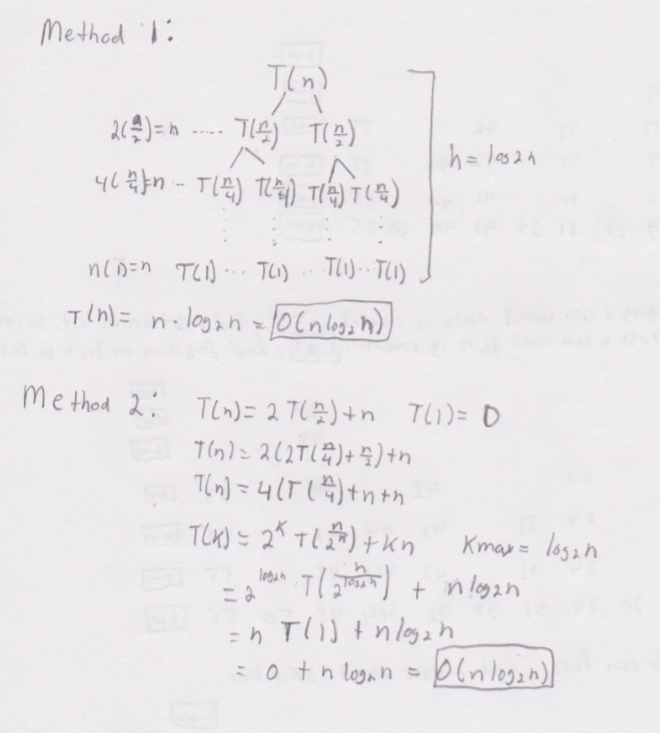
\includegraphics[scale=0.5]{6b}%
\end{minipage}
\par\end{flushleft}
\item \begin{flushleft}
What is the best, worst and average running time of the merge sort
algorithm? Justify your answer. %
\begin{minipage}[t]{1\columnwidth}%
$\newline$Merge sort does not have a best/worst/average case. In
every case it runs O($nlog_{2}n$). However, the downside is that
merge sort must use more memory because the array must be copied everytime.%
\end{minipage}\newpage{}
\par\end{flushleft}
\end{enumerate}
\item \begin{flushleft}
(10 points) R-10.17 p. 493\\
For the following statements about red-black trees, provide a justification
for each true statement and a counterexample for each false one.
\par\end{flushleft}

\begin{enumerate}
\item \begin{flushleft}
A subtree of a red-black tree is itself a red-black tree.%
\begin{minipage}[t]{1\columnwidth}%
\textbf{$\newline$Fasle. }The root of a red-black tree must be black,
however a subtree of a red-black tree may have a red root and therefore
cannot be a red-black tree%
\end{minipage}
\par\end{flushleft}
\item \begin{flushleft}
The sibling of an external node is either external or it is red.%
\begin{minipage}[t]{1\columnwidth}%
\textbf{$\newline$True. }The black depth of a node is h and the depth
of an external node is h+1 so its sibling must either a black external
node or a red node.%
\end{minipage}
\par\end{flushleft}
\item \begin{flushleft}
There is a unique (2,4) tree associated with a given red-black tree.%
\begin{minipage}[t]{1\columnwidth}%
\textbf{$\newline$True. }A node with 2 red children can be represented
by a 4-node, a node with 1 red child can be represented with a 3-node,
and a node with no red children can be represented with a 2-node.%
\end{minipage}
\par\end{flushleft}
\item \begin{flushleft}
There is a unique red-black tree associated with a given (2,4) tree.%
\begin{minipage}[t]{1\columnwidth}%
\begin{flushleft}
\textbf{$\newline$False. }A 3-node can be represented in more than
one way in a red-black tree.
\par\end{flushleft}%
\end{minipage}
\par\end{flushleft}
\end{enumerate}
\item \begin{flushleft}
(10 points) R-10.19 p. 493\\
Consider a tree $T$ storing 100,000 entries. What is the worst-case
height of $T$ in the following cases?
\par\end{flushleft}

\begin{enumerate}
\item \begin{flushleft}
$T$ is an AVL tree.%
\begin{minipage}[t]{1\columnwidth}%
$\newline$$1.44log_{2}(100000+1)=1.44log_{2}(100001)=23.9179032\approx24$.
The worst case height of a AVL tree with 100000 elements would be
24.%
\end{minipage}
\par\end{flushleft}
\item \begin{flushleft}
$T$ is a (2,4) tree.%
\begin{minipage}[t]{1\columnwidth}%
$\newline$$log_{2}(100000+1)=log_{2}(100001)=16.609655\approx17$.
The worst case height of a (2-4) tree with 100000 elements would be
17.%
\end{minipage}
\par\end{flushleft}
\item \begin{flushleft}
$T$ is a red-black tree.%
\begin{minipage}[t]{1\columnwidth}%
$\newline$$2log_{2}(100000+1)=2log_{2}(100001)=33.21931\approx33$.
The worst case height of a red-black tree with 100000 elements would
be 33.%
\end{minipage}
\par\end{flushleft}
\item \begin{flushleft}
$T$ is a binary search tree.%
\begin{minipage}[t]{1\columnwidth}%
$\newline$The worst case height for a binary search tree is O(n)
(linear binary search tree). Therefore for 100000 elements, the worst
case height is 100000.%
\end{minipage}\newpage{}
\par\end{flushleft}
\end{enumerate}
\item \begin{flushleft}
(10 points) R-9.16 p. 418
\par\end{flushleft}


\begin{flushleft}
Draw an example skip list that results from performing the following
series of operations on the skip list shown in Figure 9.12: \texttt{erase(}38\texttt{),
insert(}48,x\texttt{), insert(}24,y\texttt{), erase(}55\texttt{)}.
Record your coin flips, as well.$\newline\newline$%
\begin{minipage}[t]{1\columnwidth}%
\begin{flushleft}
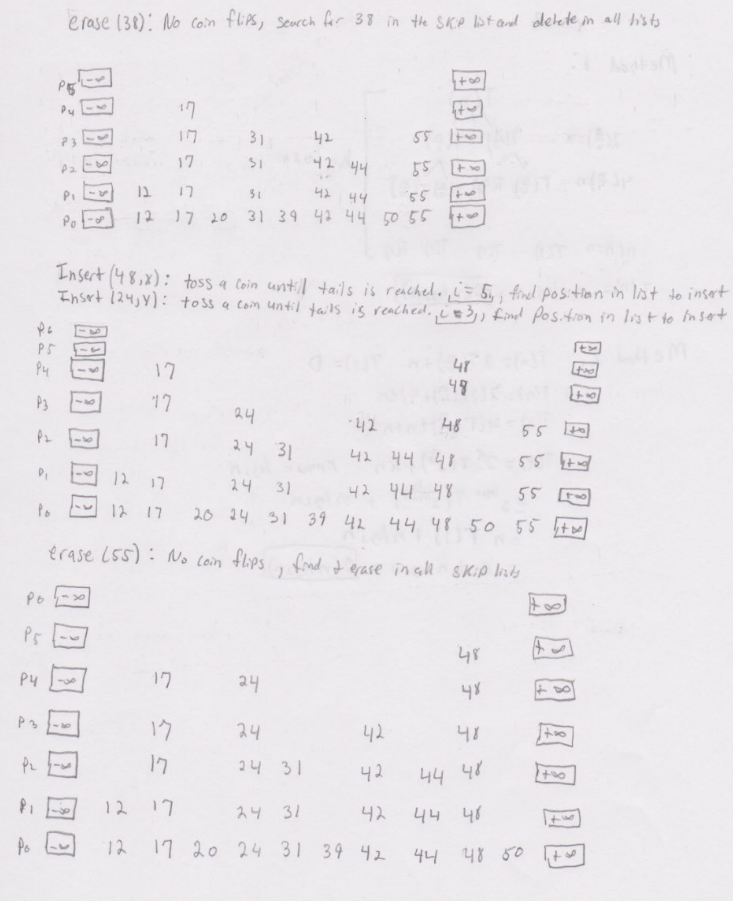
\includegraphics[scale=0.75]{9}
\par\end{flushleft}%
\end{minipage}\newpage{}
\par\end{flushleft}

\item \begin{flushleft}
(10 points) R-9.7 p. 417
\par\end{flushleft}


\begin{flushleft}
Draw the 11-entry hash table that results from using the has function,
$h(k)=(3k+5)$ mod 11, to hash the keys 12, 44, 13, 88, 23, 94, 11,
39, 20, 16, and 5, assuming collisions are handled by chaining.$\newline\newline$%
\begin{minipage}[t]{1\columnwidth}%
\begin{flushleft}
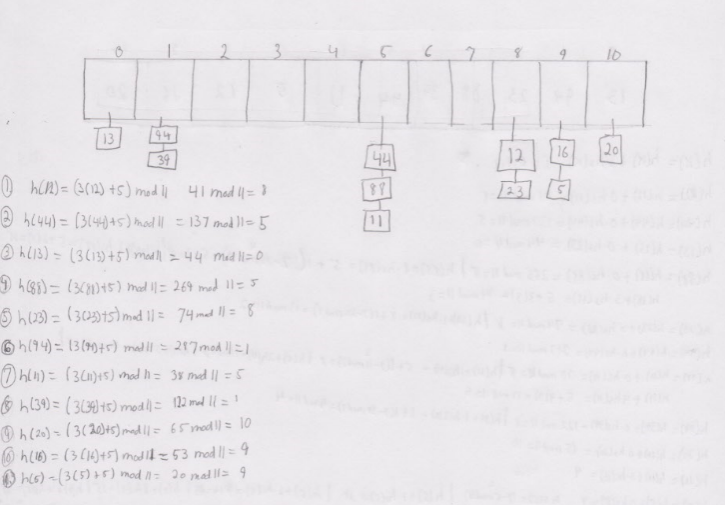
\includegraphics[scale=0.75]{10}
\par\end{flushleft}%
\end{minipage}
\par\end{flushleft}

\item \begin{flushleft}
(10 points) R-9.8 p. 417
\par\end{flushleft}


\begin{flushleft}
What is the result of the previous exercise, assuming collisions are
handled by linear probing?$\newline\newline$%
\begin{minipage}[t]{1\columnwidth}%
\begin{flushleft}
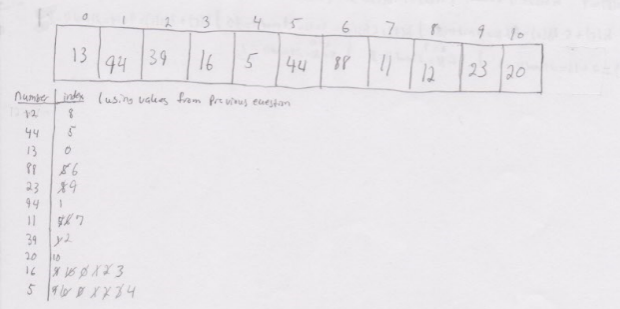
\includegraphics{11}$\newline$
\par\end{flushleft}%
\end{minipage}\newpage{}
\par\end{flushleft}

\item \begin{flushleft}
(10 points) R-9.10 p. 417 
\par\end{flushleft}


\begin{flushleft}
What is the result of Exercise R-9.7, when collisions are handled
by double hashing using the secondary hash function $h_{s}(k)=7-(k$
mod $7)$?$\newline\newline$%
\begin{minipage}[t]{1\columnwidth}%
\begin{flushleft}
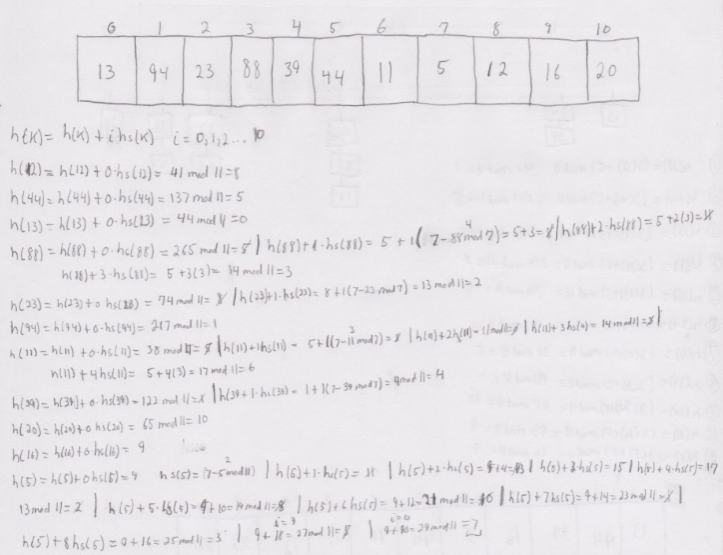
\includegraphics[scale=0.75]{12}$\newline$
\par\end{flushleft}%
\end{minipage}
\par\end{flushleft}

\end{enumerate}
\begin{flushleft}

\par\end{flushleft}
\end{document}
